This section presents the results of the experiments conducted in this project. The experiments were designed to evaluate the performance of the DSU process in the context of embedded systems, and to investigate the impact of using FRAM as the storage medium for the update process. The main focus of the experiments was to measure the time it takes to perform the update process, and evaluate if the procedure is feasible in a real-time system.

All of the below experiments were conducted on the Texas Instruments MSP430FR5994 microcontroller, running at various clock frequencies. The data was gathered using the built-in debugging tools of the Code Composer Studio IDE. The time estimates were not measured directly but instead calculated based on the number of clock cycles spent in each part of the update process. 

\section{Simulated Updates}
As an in depth performance evaluation of the DSU process, a series of simulated updates were conducted. The simulated updates were designed to test the performance of the DSU process under various conditions, such as different update sizes, and using different clock frequencies. The simulated updates were conducted by manually creating \textit{diff} files and applying them to a preallocated array in the upper FRAM of the device. The simulated updates uses only one operation type each, to measure the impact of each operation. In the first series of experiments, the focus is to determine the bottlenecks of the process, as well as how to structure the \textit{diff} files to optimise performance. The second series of experiments focus on the clock frequency of the device, an important factor in deciding the usefulness of FRAM as the storage medium for the device.
\subsection{Decode and apply performance}
\todo{Emphasize apply phase}
\subsubsection*{\textbf{\textit{Decode phase}}}
Figure \ref{fig:wDecode8} shows the processor cycles required to decode \textbf{Write} operations at different update sizes running at 8MHz. The cycles required to decode the operation is linear with the size of the update, and grows at an increasingly higher rate the more operations are used, as shown by the "1 op / Word" data points. This 'context switching' overhead is sizeable, adding triple the amount of cycles compared to extending a single operation with another word of data. This underlines the importance of minimizing the number of operations in an update.
\begin{figure}[!ht]
    \begin{shaded}
        \centering
        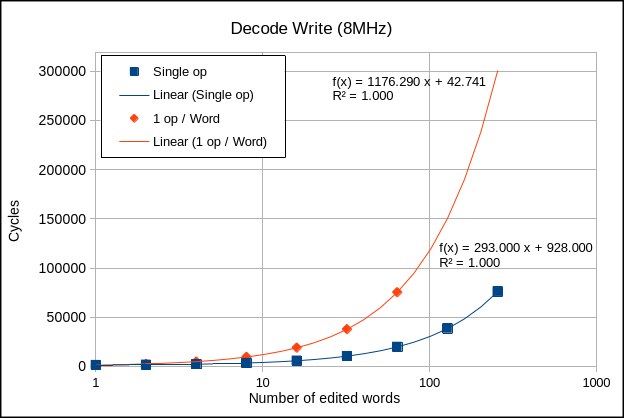
\includegraphics[width=\figurewidth]{img/WDecode8.png}
        \caption{Cycles required to decode \textbf{Write} operations running at 8MHz.}
        \label{fig:wDecode8}
    \end{shaded}
\end{figure}
The maximum update size tested was 256 words for a single operation, and a maximum of 64 operations at one word each. This is a limitation owing to the small amount of available SRAM on the device, limiting the size of the \textit{diff} file. Potential solutions to this limitation are discussed in Section \ref{sec:future_work}. 

Similarly to the \textbf{Write} operation, effort should be made to minimize the number of \textbf{Shift} operations for any given update. This is shown in figure \ref{fig:sDecode8}, where the number of cycles required to decode the operations grows even more rapidly with the number of operations. This, however, is not as critical as the \textbf{Write} operation, as the number of \textbf{Shift} operations is expected to be lower than the number of \textbf{Write} operations for a given update. 
\begin{figure}[!ht]
    \begin{shaded}
        \centering
        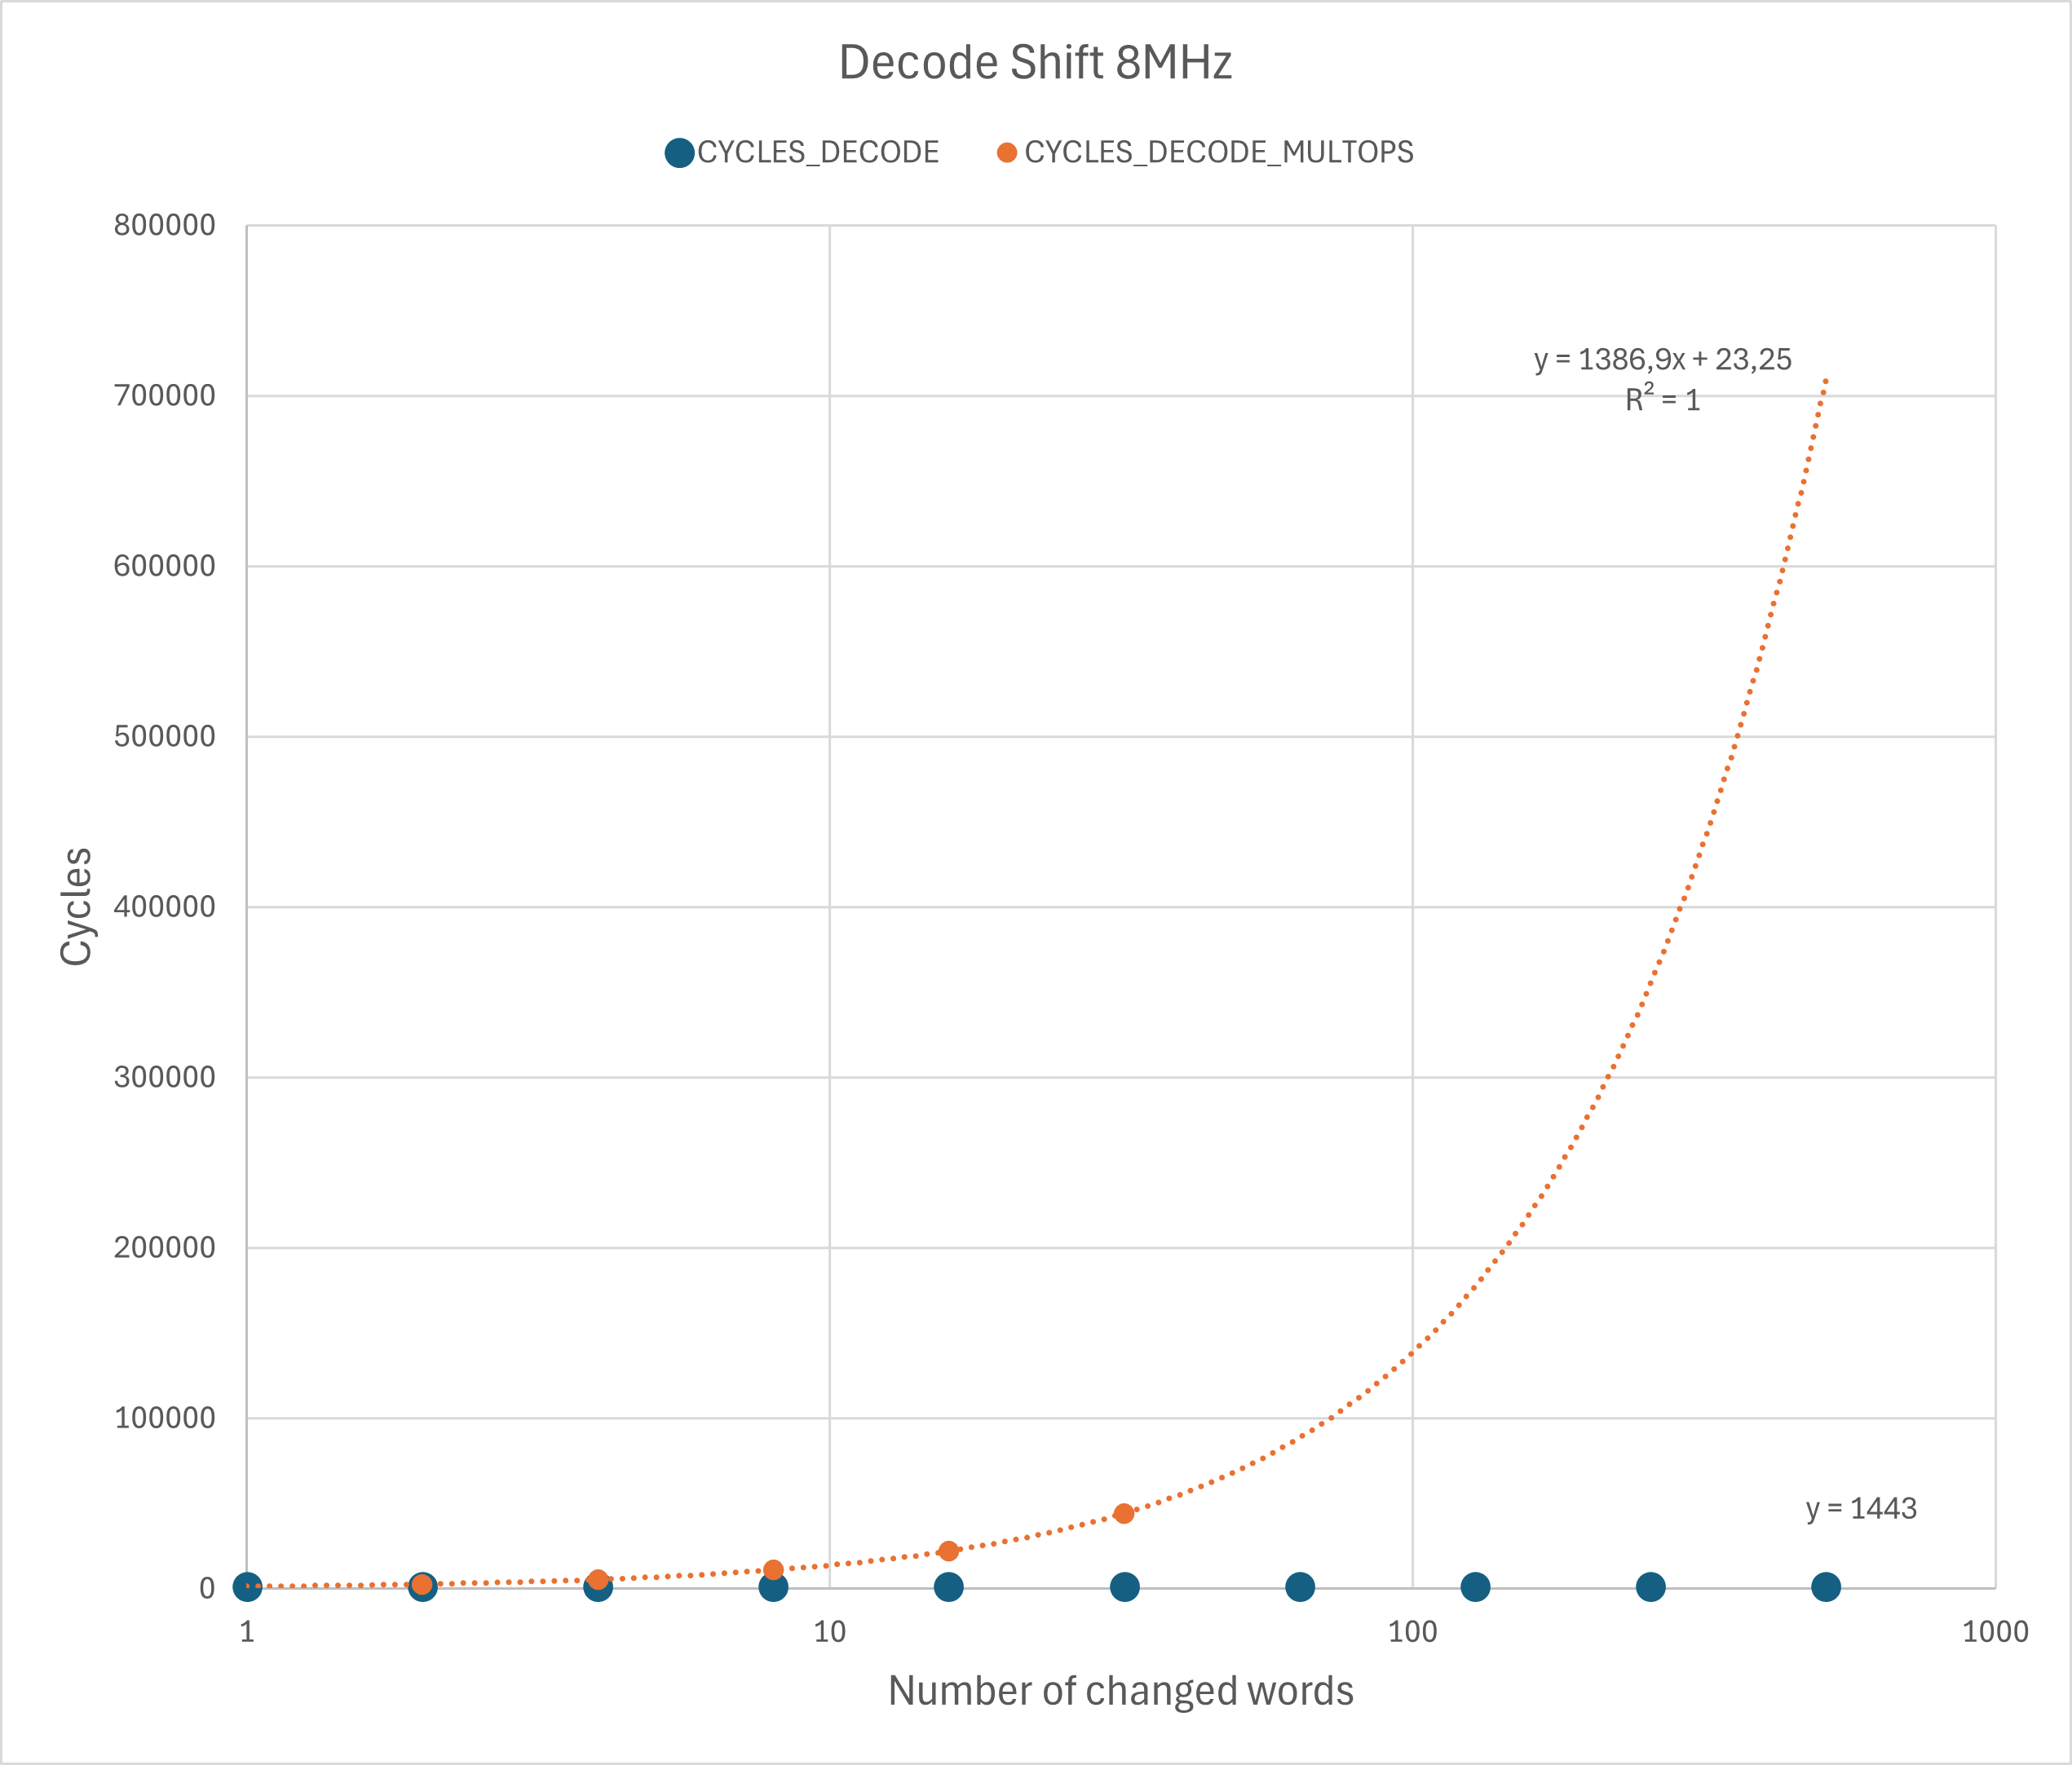
\includegraphics[width=\figurewidth]{img/SDecode8.png}
        \caption{Cycles required to decode \textbf{Shift} operations running at 8MHz.}
        \label{fig:sDecode8}
    \end{shaded}
\end{figure}
Again, the available RAM of the device limited the maximum update size tested to just 32 operations. 

The results of the simulated updates show that the decode phase is very taxing on the processor, and that the number of operations in an update has a significant impact on the time it takes to decode the update. The main focus of this research however, is the impact that the FRAM has on the performance of the update process. this is more clearly shown in the apply phase, where the use of, for example, Flash would bring a severe performance penalty.

\subsubsection*{\textbf{\textit{Apply phase}}}
Figure \ref{fig:wApply8} shows the \textit{application} of the previously discussed updates. The cycles required to apply the updates is also linear with the size of the update, but the rate of growth is significantly lower than that of the decode phase.
\begin{figure}[!ht]
    \begin{shaded}
        \centering
        \includegraphics[width=\figurewidth]{img/wApply8.png}
        \caption{Cycles required to apply \textbf{Write} operations running at 8MHz.}
        \label{fig:wApply8}
    \end{shaded}
\end{figure}
Here, a view of the improvement over traditional storage mediums can be seen. Using numbers from the data sheet for similar platforms from Texas Instruments, which use Flash \cite{msp430Flash}, the maximum speed for pre-erasing 512 bytes of data on Flash is 23ms, or an estimated 11.5ms for 256 bytes. This is well beyond the real-time deadlines which researchers such as Yaacoub et al. have shown to be realistic \cite{NeRTA}, and does not include the time it takes to write the data. In comparison, the DSU process using FRAM can write this data in just 0.44ms, as estimated from the data in figure \ref{fig:wApply8}.

The \textbf{Shift} operation behaves identically when it comes to the apply phase, as seen in figure \ref{fig:sDecodeVsApply}. The growth of 12 cycles for each additional edited word, with a fixed decode cost, means the \textbf{Shift} operation allows updates which shift large portions of the code without significant performance costs. Using the linear equation from the figure, $f(x)=12x+134$, an approximate 1988 words, or 3976 bytes could be written or shifted within 3ms. 
\begin{figure}[!ht]
    \begin{shaded}
        \centering
        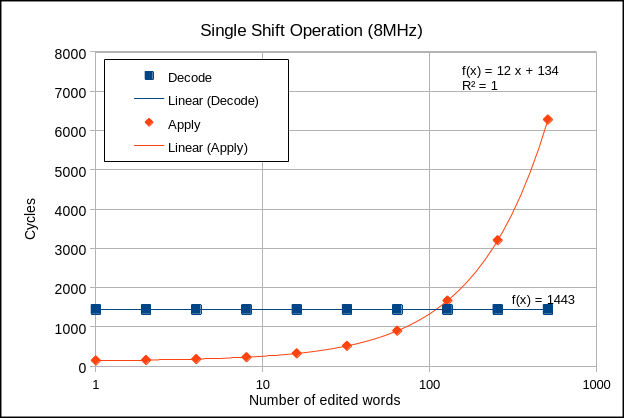
\includegraphics[width=\figurewidth]{img/SDecodeVsApply.png}
        \caption{Comparison of Decode and Apply phases for a single \textbf{Shift} operation running at 8MHz.}
        \label{fig:sDecodeVsApply}
    \end{shaded}
\end{figure}
Additional tests were made to verify that the \textit{offset} of the \textbf{Shift} operation does not impact the performance, and the results showed that this is indeed the case. 

\subsection{Clock frequency impact}
As previously mentioned, the MSP430FR5994 is limited to 8MHz when accessing FRAM. This means running the device at 16MHz will require wait states for every access to FRAM. Although this introduces some overhead in the form of additional cycles required for each access, the overall real-time performance of the update process is should still be improved owing to the faster processing of data.  
In Figure \ref{fig:w8vs16}, the difference in required cycles can be seen when running the same update at different clock frequencies. Even with the added overhead of wait state cycles, the update process is faster at 16MHz than at 8MHz, running at twice the speed but with, on average, $22.9\%$ more cycles required. 
\begin{figure}[!ht]
    \begin{shaded}
        \centering
        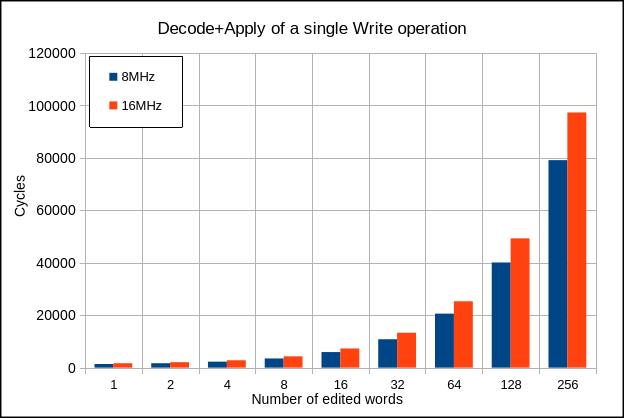
\includegraphics[width=\figurewidth]{img/W8vs16.png}
        \caption{Comparison of cycles required to decode and apply \textbf{Write} operations running at 8MHz and 16MHz.}
        \label{fig:w8vs16}
    \end{shaded}
\end{figure}

In previous works related to this, various real-time deadlines have been targeted, such as Wahler et al. with 5ms \cite{dynUpdateFramework}, and Yaacoub et al. who measured an idle time of 3ms. Thus, these numbers ase used as target deadlines for the following discussion. Note that these deadlines may differ dramatically depending on the application and target system. 

The results of the simulated updates show that the DSU process benefits greatly from a higher clock frequency. 
\todo{Stack decode + apply on top of eachother}
\begin{figure}[!ht]
    \begin{shaded}
        \centering
        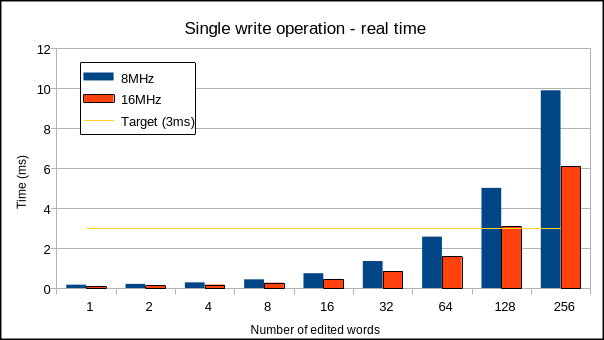
\includegraphics[width=\figurewidth]{img/W8vs16_rt.png}
        \caption{Comparison of real time required to decode and apply \textbf{Write} operations running at 8MHz and 16MHz.}
        \label{fig:s8vs16}
    \end{shaded}
\end{figure}

In figure \ref{fig:s8vs16}, the real-time performance of the update process is shown. The real-time performance is calculated by multiplying the number of cycles required to perform the update with the clock cycle time. As can be seen, the real-time performance of the update process is significantly improved when running at 16MHz, with the update process being on average $38.6\%$ faster. This is a significant improvement, and shows that the DSU process is feasible in a real-time system, even with the added overhead of wait states. Furthermore, using a linear regression, an estimated maximum size of a write operation was calculated to 124 words at 16MHz while still meeting the 3ms deadline. At 8MHz, this number is instead 75 words. This includes the decode phase, which the majority of time is spent in. Thus, if future work improves upon the decode phase, perhaps with more sophisticated encoding, it would certainly be possible to increase this limit.

\todo{shift operation}
\section{Proof of Concept Updates}
Firstly, to demonstrate the feasibility of the DSU process, a simple update was constructed which changes a single word in the binary image and makes the LED of the launchpad blink at a different frequency. 
\todo{data}
As expected from such a small update, the time it takes to perform the update is very short, with the majority of time spent in the decoding phase. 

As a more interesting proof-of-concept, a larger update was constructed which changes the behaviour of the LED blinking and introduces new functionality to the application. The application pre-update simply blinks both LEDs on the launchpad at a fixed, synchronized frequency. The post-update application adds functionality to a button on the microcontroller. When pressed, the button changes the blinking frequency of one of the LEDs and makes them unsynchronized, thus providing a more complex update scenario which also has the benefit of being visibly verifiable. 
\begin{framed}
\noindent\begin{minipage}{.45\textwidth}
\begin{lstlisting}[
    caption={The interrupt service routine before DSU.},
    label={lst:pre_dsu_isr}
]
if (P5IFG & BIT5)
{ // Button 1 pressed
    update(diff);
}

P5IFG &= 0; // Clear interrupt flag
\end{lstlisting}
\end{minipage}\hfill
\noindent\begin{minipage}{.45\textwidth}
\begin{lstlisting}[
    caption={The interrupt service routine after DSU.},
    label={lst:post_dsu_isr}
]
if (P5IFG & BIT5)
{ // Button 1 pressed
    update(diff);
} 
if (P5IFG & BIT6)
{ // Button 2 pressed
    green_period += 1000;
}

P5IFG &= 0; // Clear interrupt flags
\end{lstlisting}
\end{minipage}
\end{framed}\hfill

The update took a total of 6151 cycles to complete at 8MHz, with the majority of the time spent in the decode phase. The update process was completed in 0.76ms, which is well within the 3ms deadline. While this proof-of-concept is still relatively simple, requiring only a single \textbf{Shift}- and \textbf{Write} operation each, it demonstrates the potential of the DSU process. 
